\chapter{\label{chapter:3_preliminaries}Preliminaries and Methodology}

This chapter will cover all the necessary tools required for the thesis. As we are considering asynchronous shared memory systems, the first section will describe the mathematical foundation for the computational model. This will describe formal concepts such as \emph{process}, \emph{algorithm}, and \emph{Linearizability}~\cite{DBLP_journals_toplas_HerlihyW90} in concurrent systems.

In the following section, we will explore the hardware foundations of concurrent systems. Specifically, we will discuss concepts such as \emph{cache memory}, \emph{consistency memory model}, \emph{cache coherence}, and \emph{memory fences}, which are crucial for correctly implementing concurrent algorithms. We will also discuss the concept of a memory model at the programming language level and examine the Java and C++ memory models that define the allowable behavior of multithreaded programs.

Finally, we will conclude this chapter by discussing the statistical experimental methodology used to analyze program implementations and compare performance between them.

\section{\label{sec:chapter-3:computation-model}Computation Model}

In the realm of computing, concurrent computation stands as a cornerstone for achieving efficient and scalable systems. It enables the execution of multiple tasks simultaneously, which is crucial for modern software applications such as web servers and programs exploiting multi-core processors' power. However, the complexity of concurrent systems requires precise mathematical models to reason about their behavior accurately. This section will discuss the mathematical model in detail, including its multiple components and assumptions for the essential topics developed in this thesis.

We consider the standard concurrent shared memory with \(n \ge 2\) \textit{asynchronous} processes, \(p_0, \ldots, p_{n-1}\), which may \textit{crash} at any time during execution~\cite{DBLP_conf_spaa_Herlihy91,DBLP_books_daglib_0020056,DBLP_journals_toplas_HerlihyW90}. The \textit{index} of process \(p_i\) is \(i\). Processes communicate with each other by invoking \textit{atomic} instructions of base objects: either simple \R/\W, or more powerful \RMW, such as \SWAP or \CAS.

An \emph{algorithm} for a high-level concurrent object \(T\) (e.g., a queue or a stack) is a distributed algorithm \(\mathcal{A}\) consisting of local state machines \(A_1,\ldots, A_n\). Local machine \(A_i\) specifies which instruction of base objects execute to return a response when it invokes a (high-level) operation of \(T\); each of these instructions is a \emph{step}.

An \emph{execution} of \(\mathcal{A}\) is a (possibly infinite) sequence of steps, namely, instructions of base objects, plus invocations and responses of (high-level) operations of the concurrent object \(T\) with the following properties:

\begin{enumerate}
    \item Each process first invokes an operation, and only when it has a corresponding response can it invoke another operation, i.e., executions are well-formed and
    \item For any invocation to an operation \(op\) of a process \(p_i\), denoted as \(inv_i(op)\), the steps of \(p_i\) between that invocation and its correspondent response (if there is one), denoted \(res_i(op)\), are the steps specified by \(A_i\) when \(p_i\) invokes \(op\).
\end{enumerate}

An operation in an execution is \emph{complete} if both its invocation and response appear in the execution. An operation is \emph{pending} if only its invocation appears in the execution. It is assumed that after a process completes an operation, it non-deterministically picks the operation it executes next. An execution \(E\) is an \emph{extension} of an execution \(F\), if \(E\) is a prefix of \(F\), namely, \(E = F\cdot F'\) for some \(F'\).

For any finite execution \(E\) and any process \(p_i\), \(E|p_i\) denotes the sequence of invocations and responses of \(p_i\) in \(E\). Two finite executions \(E\) and \(F\) are equivalent if \(E|p_i = F|p_i\) \(\forall p_i\). For any execution \(E\), \(comp(E)\) denotes the execution obtained by removing from \(E\) all steps and invocations of pending operations.

A process is \emph{correct} in an infinite execution if it takes infinitely many steps. An implementation is lock-free if, in every infinite execution, infinitely many operations are complete~\cite{DBLP_journals_toplas_HerlihyW90}. An implementation is \emph{wait-free} if, in every infinite execution, every correct process completes infinitely many operations~\cite {DBLP_journals_toplas_Herlihy91}. Thus, a wait-free implementation is lock-free but not necessarily vice-versa. \emph{Bounded wait-freedom}~\cite{DBLP_conf_spaa_Herlihy91} additionally requires a bound on the number of steps needed to terminate. The \emph{step complexity} is the maximum number of steps a process needs to execute to return. The step complexity of an algorithm is the maximum among the step complexity of its operations.

In the \RAW{} synchronization pattern, a process first writes in a shared variable and then reads another shared variable, maybe executing other instructions in between. For example, this mechanism is widely used in the classic Lamport's bakery mutual exclusion algorithm (see~\cite {DBLP_books_daglib_0020056}). The correctness of the mechanism requires that the write and read instructions of a process are executed in a specific order, although there is no data dependence relation between them. In Section~\ref{sec:hardware-foundations}, we will discuss thoroughly how current processor architectures can reorder instructions, how they can alter the correctness of concurrent algorithms, and how to avoid this problem using \emph{fences}.

An algorithm, or one of its operations, is \emph{fence-free} if it does not require any specific ordering among its steps beyond what is implied by data dependence (e.g., the value written by a \W{} instruction depends on the value read by a previous \R instruction). Note that a fence-free algorithm does not use \RAW{} synchronization patterns. In our algorithms, we use notation \(\{O_1.inst_1, \ldots, O_x.inst_x\}\) to denote that the instructions \(O_1.inst_1, \ldots, O_x.inst_x\) can be executed in any order. Observe that memory fences (also known as memory barriers) are not required to correctly implement a fence-free algorithm in a concrete language or multi-core architecture since any reordering of non-data-dependent instructions does not affect the correctness of the algorithm.

\emph{Linearizability}~\cite{DBLP_journals_toplas_HerlihyW90} is the standard correctness condition for concurrent objects. Intuitively, an execution is linearizable if its (high-level) operations can be ordered sequentially, without reordering non-overlapping operations, so that their responses satisfy the specification of the implemented object.

A \emph{sequential specification} of a concurrent object \(T\) is a state machine specified through a transition function \(\delta\). Given a state \(q\) and an invocation \(inv_i(op)\) of process \(p_i\), \(\delta(q, inv_i(op))\) returns the tuple \((q', res_i(op))\) (or a set of tuples if the machine is \emph{non-deterministic}) indicating that the machine moves to state \(q'\) and the response to \(op\) is \(res_i(op)\). The sequences of invocation-responses tuples \(\langle inv_i(op): res_i(op)\rangle\) produced by the state machine are its \emph{sequential executions}. For the sake of clarity, a tuple \(\langle inv_i(op): res_i(op)\rangle\) is simply denoted \(op\). Also, the subscripts of invocations and responses are omitted.

Given an execution \(E\), we write \(op <_E op'\) if and only if \(res(op)\) precedes \(inv(op')\) in \(E\). Two operations are \emph{concurrent} denoted \(op||_E op' \), if neither \(op <_e op'\) nor \(op' <_E op\). The execution is sequential if \(<_E\) is a total order.

\begin{definition}[Linearizability~\cite{DBLP_journals_toplas_HerlihyW90}]
Let be \(\mathcal{A}\) an algorithm for a concurrent object \(T\). A finite execution \(E\) of \(\mathcal{A}\) is \emph{linearizable with respect to \(T\)}, or just \emph{linearizable} if \(T\) is clear from the context, if there is a sequential execution \(S\) of \(T\) and \(E\) can be extended to an execution \(E'\) by appending zero or more responses such that:

\begin{enumerate}
    \item \(comp(E')\) and \(S\) are equivalent and
    \item for every two complete operations \(op\) and \(op'\) in \(E\), if \(op <_E op'\) then \(op <_S op'\).
\end{enumerate}

We say that \(\mathcal{A}\) \emph{is linearizable with respect to} \(T\) or just \emph{linearizable} if \(T\) is clear from the context if each of its executions is linearizable.
\end{definition}

Another correctness condition for concurrent objects is \emph{Set-Linearizability}. Set-Linearizability~\cite{DBLP_journals_jacm_CastanedaRR18, DBLP_conf_podc_Neiger94} is an extension of linearizability, allowing multiple operations to be linearized at the same linearization point, whereas linearizability requires a total order of operations.


A \emph{set-sequential specification} of a concurrent object differs from a sequential execution in that \(\delta\) receives as input the current state \(q\) of the machine and set \(Inv = \{inv_{id_1}(op_1), \ldots, inv_{id_t}(op_t)\}\) of operation invocations, and \(\delta(q, Inv)\) returns \((q', Res)\), where \(q'\) is the next state and \(Res = \{res_{id_1}(op_1), \ldots, res_{id_t}(op_t)\}\) are the responses to the invocations in \(Inv\) and each \(id_i\) denotes the index of the invoking/responding process. Intuitively , all operations \(op_1, \ldots, op_t\) are performed concurrently and move the machine from state \(q\) to \(q'\). The sequence of sets \(Inv\), \(Res\) is a \emph{concurrency class} of the machine. The state machine's sequences of concurrency classes are its \emph{set-sequential executions}. In our set-sequential specifications, invocations will be subscripted with the index of the invoking process only when there is more than one invocation in a concurrency class. Observe that a set-sequential specification in which all concurrency classes have a single element corresponds to a sequential specification.

Given a set-sequential execution \(S\) of a set-sequential object, the partial order \(<_S\) on the operations of \(S\) is defined as above: \(op <_S op'\) if and only if \(res(op)\) precedes \(inv(op')\) in \(S\), namely, the concurrency class of \(op\) appears before of the concurrency class of \(op'\).

\begin{figure}[!ht]
  \centering
  \subfloat[\label{fig-example-linear}Linearizability]{
    {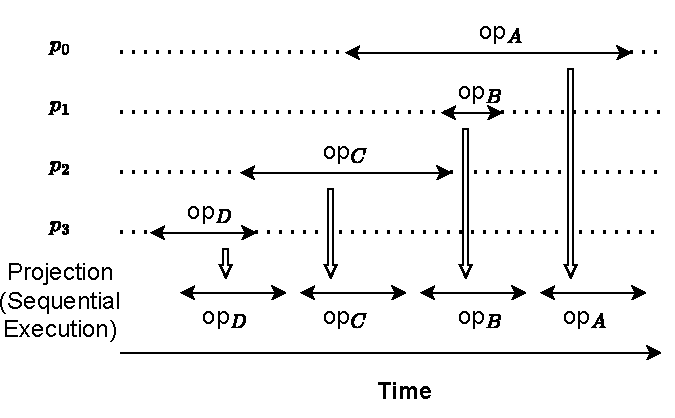
\includegraphics[width=0.47\textwidth]{contents/figures/III_1_linearizability}}
  }\hfill
  \subfloat[\label{fig-example-set-linear}Set-Linearizability]{
    {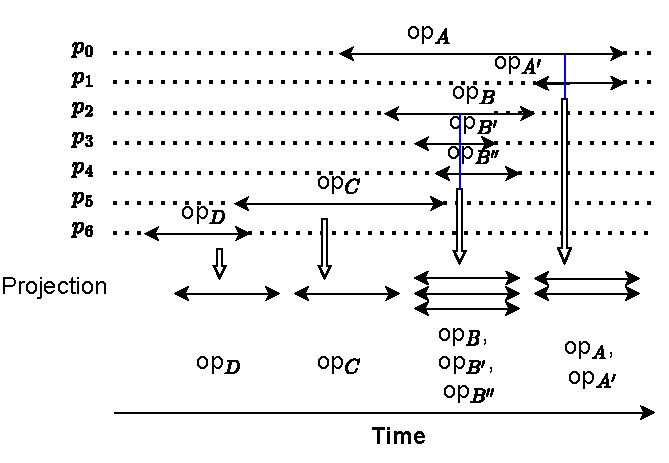
\includegraphics[width=0.47\textwidth]{contents/figures/III_1_set_linearizability}}
  }
  \caption{\label{fig-example-linear-and-set-linear}Graphical
    description of linearizability and set-linearizability.
}
\end{figure}


\begin{definition}[Set-linearizability~\cite{DBLP_journals_jacm_CastanedaRR18, DBLP_conf_podc_Neiger94}]
    Let be \(\mathcal{A}\) an implementation of a concurrent object \(T\). A finite execution \(E\) of \(\mathcal{A}\) is \emph{set-linearizable with respect to} \(T\), or just \emph{set-linearizable} if \(T\) is clear from the context, if there is a set-sequential execution \(S\) of \(T\) and \(E\) can be extended to an execution \(E'\) by appending zero or more responses such that:

    \begin{enumerate}
        \item \(comp(E')\) and \(S\) are equivalent,
        \item for every two completed operations \(op\) and \(op'\) in \(E\), if \(op <_E op'\) then \(op <_S op'\).
    \end{enumerate}

    We say that \(\mathcal{A}\) is \emph{set-linearizable with respect to} \(T\), or just \emph{set-linearizable} if \(T\) is clear from the context if each of its executions is set-linearizable.
  \end{definition}

A comparison between Linearizability and Set-Linearizability can be found in Figures~\ref{fig-example-linear} and~\ref{fig-example-set-linear}, respectively.

\section{\label{sec:hardware-foundations}Hardware Foundations}

Knowing the hardware foundations behind concurrent computing besides the mathematical computation model is important. When we translate concurrent algorithms from the mathematical computation model to a program in a particular programming language, we need to deal with a lot of assumptions and rules that do not necessarily current processor architectures follow. For example, when we design our algorithms, we suppose linearizability is the correctness condition in asynchronous shared memory. Still, current processors cannot implement linearizability in the real world because this property incurs significant costs\footnote{For example, high power consumption, high manufacturing cost, low performance, etc.}. Instead of stronger correctness conditions for asynchronous shared memory, manufacturers provided distinct types of memory consistency (also known as memory model)~\cite{DBLP_series_synthesis_2020Nagarajan, DBLP_series_synthesis_2013Scott} for their processors and machines. A memory model is a precise, architecturally visible definition of shared memory correctness~\cite{DBLP_series_synthesis_2020Nagarajan}. Knowing about the hardware foundations helps us to implement correct algorithms. This will help us understand why specific tools like ``\emph{fences}'' are necessary to ensure correct concurrent computing. In this section, we will discuss the functioning of concurrent programs on computer hardware at a high level and focus on memory interactions at various levels.

\begin{figure}[ht!]
    \centering
    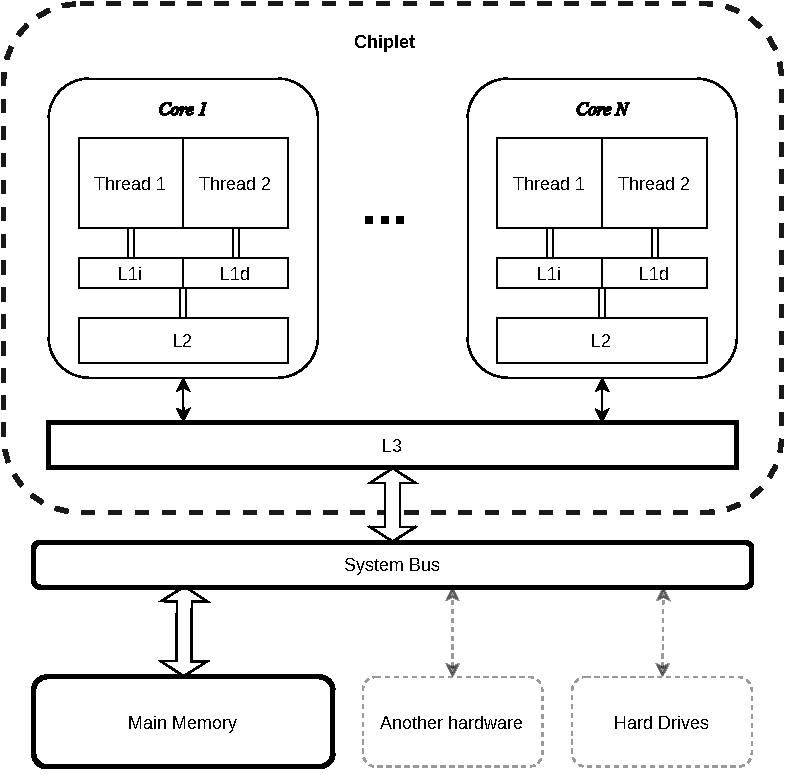
\includegraphics[width=0.7\linewidth]{contents//figures/III_2_cpu.pdf}
    \caption{Baseline model of a Multi-core Processor Chip.}
    \label{fig:multi-core-processor}
\end{figure}

When analyzing computer systems, it is important to consider those with multi-core processors communicate through a shared memory. This means all cores in the processor, can perform reads (loads) and writes (stores) to all addresses in the memory. A typical system model includes a single chip with multiple cores and off-chip main memory. You can see an illustration of this model in the figure~\ref{fig:multi-core-processor}\footnote{In the figure~\ref{fig:multi-core-processor}, we omit many features to simplify the reasoning about the hardware}. Usually, a multi-core processor includes \emph{cache memory}, a special high-speed memory close to the processor that allows fast process access. Caches decrease the average latency when accessing storage structures~\cite{DBLP_series_synthesis_2020Nagarajan, DBLP_series_synthesis_2013Scott}. In recent times, multi-core chips have adopted a three-tiered cache memory system. Each core has its own private L1 and L2 cache levels, while all the cores share the L3 cache level. The primary purpose of the cache levels L1 and L2 is to provide fast access to data and instructions for the core. Each core uses the first cache level to retrieve required data and execute instructions. Cache L1 is divided into two sub-caches, one for data (L1d) and the other for instructions (L1d). Typically, access to this cache level is faster than access to other levels. The second level of cache is usually more extensive and stores data and instructions about to be executed.
Multiple cores share the third cache level and serve as a source for the L2 cache~\cite{devices_amd64,guideintel}.


The \emph{main memory} holds frequently accessed data for the CPU, such as instructions or processing data, and allows faster access than secondary memory. The processor calls the \emph{memory bus} to obtain such data and instructions, which transfers data from the primary memory to the CPU and cache memory. This bus has three parts: the address bus, the control bus, and the data bus. The address bus is used to retrieve information about the location of stored data.  On the other hand, the control bus is utilized to transfer control signals from control units to other components of the computer. Finally, the data bus transfers information between the primary memory and the corresponding chipset.


When considering the simplified view of cache and memory architecture, it is important to ensure that shared memory is correct. Incoherence can occur when multiple actors have concurrent access to caches and memory, such as processor cores, external devices, system buses, etc., which may read and/or write to them. The cores will be the main actors, but we must consider the possibility of other actors interacting with caches and memory.

In order to ensure that shared memory is accurate, two important issues must be addressed: \emph{consistency} and \emph{correctness}. Consistency establishes rules for how memory reads (loads) and writes (stores) interact with the memory. These rules must consider the behavior of these operations when multiple threads or even a single thread accesses memory. Consistency models define the proper behaviors for shared memory about loads and stores and do not reference caches or coherence~\cite{DBLP_series_synthesis_2020Nagarajan}. Memory consistency models (or memory models) specify shared memory correctness. They define the allowed behaviors for multithreaded programs that execute with shared memory. The most intuitive and strongest memory model is \emph{Sequential Consistency} (SC)~\cite{lamport1979how}. Another memory model used by systems \emph{x86} and \emph{SPARC} is \emph{Total Store Order} (TSO) ~\cite{DBLP_conf_tphol_OwensSS09, DBLP_journals_cacm_SewellSONM10, sparc1992sparc}. TSO is driven by the goal of utilizing \emph{first-in-first-out} write buffers to store the outcomes of completed stores prior to writing the results to the caches. Additionally, ``relaxed'' or ``weak'' memory models are considered because they show that most memory orderings in strong models are unnecessary~\cite{DBLP_series_synthesis_2020Nagarajan}.


It is important to consider cache coherence protocols when dealing with caching and solving coherence issues. These protocols come into play when multiple cores access multiple copies of data, with at least one being a write access. To ensure that the data accessed is up-to-date and consistent, the distributed set of cores implements a set of rules within a system~\cite{DBLP_series_synthesis_2020Nagarajan}. Hence, it is essential to consider consistency models and cache coherence protocols to prevent access to stale or incoherent data. The goal of a coherence protocol is to maintain coherence by enforcing the next invariants~\cite{DBLP_series_synthesis_2020Nagarajan}:

\begin{enumerate}
  \item \emph{Single Writer, Multiple-Read Invariant} \texttt{(SWMR)}. At any given
 (logical) time, only one core may write to memory location \(A\). Other cores may only read the memory location \(A\).

  \item \emph{Data-Value Invariant}. The value of the memory location at the beginning of an epoch is the same as the value of the memory location at the end of its last read-write epoch.
\end{enumerate}

To ensure that the \texttt{SWMR} and \emph{data value} invariants are always maintained, we use a distributed system consisting of a collection of \emph{coherence controllers}. Such controllers are finite state machines associated with each storage structure (cache and memory). These coherence controllers exchange messages with each other to ensure that invariants are upheld for each structure. The coherence protocol specifies the interaction between these finite-state machines and moving from one state to another based on the conditions of the data and the cache memory~\cite{DBLP_series_synthesis_2020Nagarajan}.

The coherence controllers have several important responsibilities. They handle service requests from two sources: Core and Network. On the ``Core side'', the cache controller interfaces with the processor core, receiving loads and stores from the core and returning load values to the core. Additionally, the cache controller initiates coherence transactions by issuing a coherence request in the case of a cache miss. This coherence request is sent to one or more coherence controllers across the interconnection network~\cite{DBLP_series_synthesis_2020Nagarajan}. On the cache controller's ``network side'', it interfaces with the rest of the system through the interconnection network. The controller receives requests and coherence responses that it must process~\cite{DBLP_series_synthesis_2020Nagarajan}. A coherence controller is illustrated in Figure~\ref{fig:cache_controller}.

\begin{figure}[ht]
  \centering
  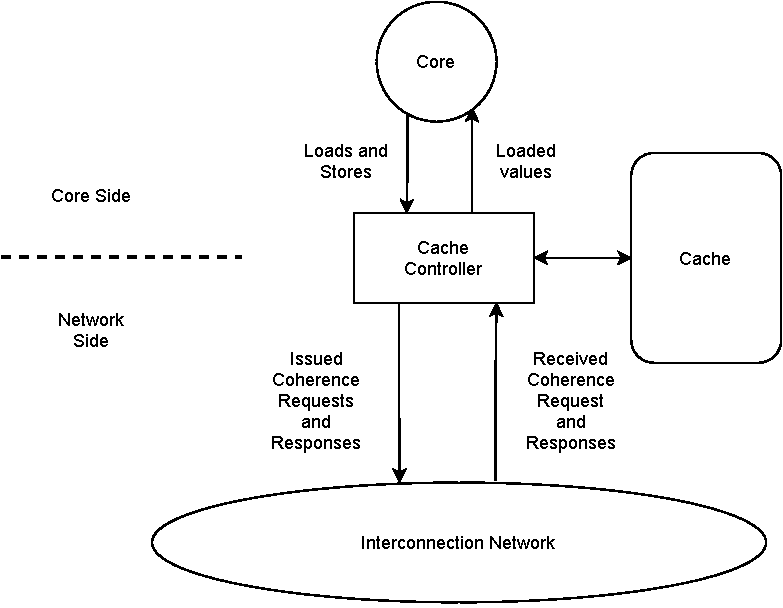
\includegraphics[scale=0.9]{contents/figures/III_3_Cache_Controller.pdf}
  \caption{\label{fig:cache_controller}Cache Controller}
\end{figure}


Coherence states are essential for ensuring the smooth operation of a system. These states assist the coherence controller in deciding whether it needs to communicate with other controllers to retrieve new data, update existing data, or continue operating with the current data. The most commonly used coherence states are modified (M), shared (S), and invalid (I). However, AMD has gone a step further with its MOESI protocol~\cite{devices_amd64} and introduced two additional states, owned (O) and exclusive (E), to improve the system's efficiency. On the other hand, Intel has created its extension called MESIF~\cite{guideintel} to achieve the same goal. A detailed explanation of how coherence protocols work can be found in the book of Nagarajan et al. ~\cite{DBLP_series_synthesis_2020Nagarajan}.

\section{About Fences And Its Use In Concurrent Algorithms}

In many processor architectures, it is common to see cores reordering memory accesses to different addresses to perform efficient computations according to certain rules~\cite{DBLP_series_synthesis_2020Nagarajan}. These reorders do not affect the execution of a single-thread program. We can consider three possible reorder cases: load-load, store-store, and load-store or store-load. Processors that support the sequential consistency model require each core to preserve the program order in any of those combinations.

However, processors that support the TSO memory model do not guarantee ordering between a store and a subsequent load that comes after it in program order~\cite{DBLP_conf_tphol_OwensSS09, DBLP_journals_cacm_SewellSONM10}. The reason behind this is that processor cores write to store buffers to hold committed stores until the rest of the memory system can process the stores. Nevertheless, they ensure that the load gets the value of the earlier store.

Compilers can reorder instructions and memory accesses to enhance performance and reduce the cost of certain loads and stores to and from memory. In some cases, if the programmer knows what he is doing, he can use some compilation flags to indicate to the compiler to use instruction reordering, allowing data races of stores in multi-threaded environments\footnote{See, for example, the options that control optimizations in the GCC compiler, in specific the flag -Os, which enables all -O3 optimizations, but also turn on the option of \texttt{-fallow-store-data-races}: \url{https://gcc.gnu.org/onlinedocs/gcc/Optimize-Options.html}, and the discussion about its lack of clear documentation: \url{https://gcc.gnu.org/bugzilla/show_bug.cgi?id=97309}.}.
% To order these instructions, the programmer must explicitly specify that ordering by inserting a \emph{fence} instruction between the store and the subsequent load.
% The \emph{fence} instruction ensures that all instructions before it in program order are executed before any instructions after it in program order.

A widely used mechanism to avoid reordering (memory accesses, instructions) is the use of memory fences. A \emph{memory fence} is a special instruction that acts as a barrier that enforces an ordering constraint on memory operations (reads and writes) issued before and after such a memory fence. Memory fences are essential for maintaining memory order consistency in multi-threaded programming environments. This is because most modern CPUs or compilers perform performance optimizations, such as instruction reordering and speculative execution, which can lead to out-of-order execution. Memory fences ensure that memory operations are synchronized and appear to occur in the expected order, preventing potential issues caused by instruction reordering and ensuring the correctness of multi-threaded programs. Typically, these low-level code optimizations, may not significantly impact the behavior of a single-threaded program. However, in concurrent programs where multiple threads are executing simultaneously, these optimizations can lead to unexpected and hard-to-debug issues, such as race conditions and inconsistent data states. Therefore, it is crucial to be mindful of these potential impacts when developing and testing concurrent programs (See Example~\ref{ex:reordering}).

\begin{example}[Instruction re-ordering]
\label{ex:reordering}
Consider the following multi-thread program with two threads, each concurrently running on distinct cores. The first thread executes the code shown in~\ref{lst:thread1}, and the second one executes the code shown in~\ref{lst:thread2}:
\vspace{2mm}
\begin{lstlisting}[language=c++,label={lst:thread1}, caption={Code execute by thread 1 on core 1} ,captionpos=b]
while (z == 0);
print(y);
\end{lstlisting}

\begin{lstlisting}[language=c++,label={lst:thread2} ,caption={Code executed by thread 2 on core 2} ,captionpos=b]
y = 30;
z = 1;
\end{lstlisting}


In this case, we might expect that the instruction \texttt{print(y)} always prints the number 30. Nevertheless, the compiler or the CPU could change the order of the instructions for thread 2, giving, as a result, an execution where the value for \texttt{y} is \emph{undefined}, and the instructions could be interleaved as shown in the code~\ref{lst:reordering}:

\begin{lstlisting}[language=c++,label={lst:reordering},caption={Code reordered by CPU}, captionpos=b]
z = 1; // Thread 2
while (z == 0); // Thread 1
print(y); // Thread 1
y = 30; // Thread 2
\end{lstlisting}

However, this execution is sequentially consistent but is an out-of-order execution producing an undefined result. With the use of memory barriers, we can ensure that instructions do not be reordered. For example, our code could be rewritten as shown in~\ref{lst:thread1-fence} and~\ref{lst:thread2-fence}:

\begin{lstlisting}[language=c++,label={lst:thread1-fence} ,caption={Updating code~\ref{lst:thread1} to use fences.} ,captionpos=b,numbers=none]
while (z == 0);
fence();
print(y);
\end{lstlisting}

\begin{lstlisting}[language=c++,label={lst:thread2-fence},caption={Updating code~\ref{lst:thread2} to use fences.} ,captionpos=b,numbers=none]
y = 30;
fence();
z = 1;
\end{lstlisting}

Thus, the system cannot print 30 without setting \(z\) to 1 before. Using a fence between potentially problematic instructions ensures that the code executes correctly; therefore, the instruction reorders, as shown in Code~\ref{lst:reordering}, cannot occur.
\end{example}


In the case of processors that support the TSO memory model, reordering instructions is not always necessary to produce unpredictable behavior in concurrent programs. This is because the cores of the processors contain store buffers. To better understand this, consider Example~\ref{ex:tso-problem}.

\begin{example}[Dealing with store buffers]
  \label{ex:tso-problem}

  Consider the following multi-thread program with two threads, each concurrently running on distinct cores. Each core has its own store buffer. The first thread executes the code shown in~\ref{lst:tso-1}, and the second executes the code shown in~\ref{lst:tso-2}. Initially, \(x = 0\) and \(y = 0\). Is it possible that \((r1, r2) = (0, 0)\) at the end of the execution?

  \begin{lstlisting}[language=c++,label={lst:tso-1}, caption={Code execute by thread 1 on core 1} ,captionpos=b]
    S1: x = FOO;
    L1: r1 = y;
\end{lstlisting}

\begin{lstlisting}[language=c++,label={lst:tso-2}, caption={Code execute by thread 2 on core 2} ,captionpos=b]
    S2: y = BAR;
    L2: r2 = x;
\end{lstlisting}

  If we analyze the possible execution of these codes, we can identify four potential outcomes for the values of \(r1\) and \(r2\). These outcomes are \((BAR, FOO)\), \((BAR, 0)\), \((0, FOO)\), and \((0, 0)\). However, it is important to note that the last outcome is invalid in a Sequential Consistent memory model. In contrast, the TSO memory model considers the final outcome valid. One might wonder how it is possible to arrive at this value. Consider the following sequence of events:

  \begin{itemize}
    \item Core 1 executes store S1, but FOO is stored in the core's write buffer.
    \item Similarly, Core 2 executes store S2 and holds BAR in its write buffer.
    \item Afterward, both cores execute their individual reads, L1 and L2, getting the value 0, which represents the previous value of x and y.
    \item Finally, both core's write buffers update memory with FOO and BAR.
    \end{itemize}

    In the end, the result of the execute the program is \((r1, r2) = (0, 0)\), which is an invalid result in Sequential Consistency. In order to prevent undesirable results, a programmer should similarly use fences as in Example~\ref{ex:reordering}. Using Code~\ref{lst:tso-1} as a basis, we can add a fence between store S1 and load L1 to ensure that write buffers are emptied into memory and that later loads are not permitted to execute until an earlier fence has been committed. We can use a similar reasoning for Code~\ref{lst:tso-2}.

\end{example}


TSO allows for the utilization of a FIFO write buffer, which is beneficial for improving performance by hiding the latency of committed stores. However, a more advanced approach would involve using a non-FIFO write buffer that enables the coalescing of writes. This means that two stores that are not in consecutive program order can be combined and written to the same entry in the write buffer. Nonetheless, employing a non-FIFO coalescing write buffer violates TSO, as TSO mandates that stores must adhere to the program order~\cite{DBLP_series_synthesis_2020Nagarajan}.

TSO behaves similarly to Sequential Consistency, permitting only one type of reordering. Hence, the use of fences is fairly infrequent, and the implementation is not too critical. However, x86 architecture provide three types of fences: \texttt{LFENCE}, \texttt{SFENCE} and, \texttt{MFENCE}~\cite{devices_amd64,guideintel}:

\begin{itemize}
  \item \texttt{MFENCE}:\@ is a full memory fence that ensures that no later loads or stores are observable globally before any earlier loads or stores. It empties the store buffer before later loads can execute.
  \item \texttt{SFENCE}:\@ only prevents the reordering of writes (it is a store-store barrier), it works well with \textit{non-temporal stores}\footnote{Non-temporal stores means that the data being stored is not going to be read again soon (i.e., no ``temporal locality'').  \url{https://sites.utexas.edu/jdm4372/2018/01/01/notes-on-non-temporal-aka-streaming-stores/}} and other instructions listed as exceptions.
  \item \texttt{LFENCE}:\@ is designed to prevent the reordering of reads with subsequent reads and writes, effectively combining load-load and load-store barriers. However, according to x86 specification, load-load, and load-store barriers are always present. As a result, LFENCE by itself is not enough for memory ordering; however, there is a larger discussion about its use far beyond the scope of this thesis.
\end{itemize}

For consistency models that permit far more reordering, fences are used more frequently, and their implementation can significantly impact performance. In programming languages, memory models are defined to provide a consistent interface for developers to implement concurrent programs, regardless of the different hardware models provided by different processor architectures. We will delve deeper into this topic in the next section.

\section{After Hardware Foundations, What's Up About Programming Languages?}

The preceding sections introduced the foundational hardware concepts needed to comprehend the memory consistency models and cache protocols required to create accurate concurrent programs. The model discussed earlier is situated at the hardware level and low-level software. However, defining or redefining memory models for high-level languages is equally important as it creates a standardized interface between a program and any software or hardware that might modify that program. A memory model also enables us to understand how the program will behave in a multi-core environment, making it easier to reason about its behavior~\cite{DBLP_journals_cacm_AdveB10, DBLP_series_synthesis_2020Nagarajan}.

In recent years, memory models have been specified for two of the most widely used programming languages, C++~\cite{DBLP_conf_pldi_BoehmA08} and Java~\cite{DBLP_conf_popl_MansonPA05}. These models describe the expected behavior of language-level threads, locks, atomics, and \RMW{} instructions. The specifications of such memory models outline the anticipated outcomes for high-level language programmers and the capabilities that compilers, runtime systems, and hardware providers can deliver. Figure~\ref{fig:memory-models} illustrates the difference between (a) high-level and (b) low-level memory models~\cite{DBLP_series_synthesis_2020Nagarajan}.

Java and C++ adopt the relaxed memory model approach of ``\emph{Sequential Consistency for Data-Race Freedom (SC for DRF)}''~\cite{DBLP_conf_isca_AdveH90}.  A data race occurs when two memory accesses target the same location simultaneously and are not reads or synchronization operations. The approach of \emph{SC for DRF} guarantees that a program is correctly synchronized if and only if all sequentially consistent executions are free of data races. If a program is correctly synchronized, then all program executions will appear to be sequentially consistent~\cite{javamemorymodelspec}.

\begin{figure}[ht!]
    \centering
    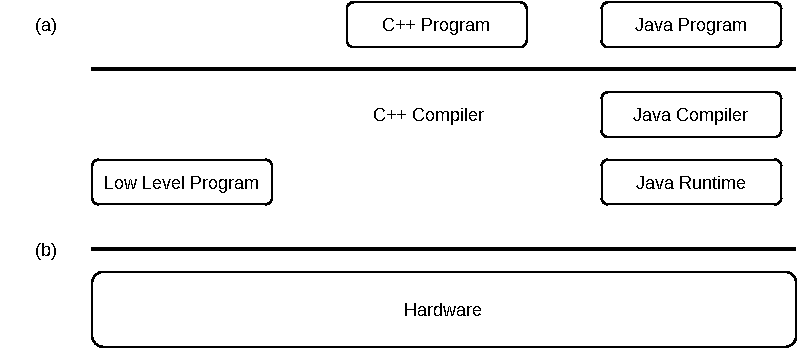
\includegraphics[width=0.9\linewidth]{contents//figures/III_3_memory_model.pdf}
    \caption{(a) High-level and (b) low-level memory models.}
    \label{fig:memory-models}
\end{figure}

The memory model of C++ specifies the order in which memory accesses, including regular, non-atomic memory accesses, should occur around an atomic operation~\cite{memoryOrderCpp2020}. Without constraints on a multi-core system, when multiple threads simultaneously read and write to multiple variables, one thread may observe the values change in a different order than the order in which another thread wrote them. This can also occur among multiple reader threads~\cite{memoryOrderCpp2020}. Similar effects can occur even on uniprocessor systems due to compiler transformations allowed by the memory model. By default, all atomic operations provided by the library follow sequentially consistent ordering. However, this default can negatively impact performance. The library's atomic operations can be given an additional memory order argument to specify precise constraints beyond atomicity that the compiler and processor must enforce for a specific operation~\cite{memoryOrderCpp2020}. This argument specifies the precise constraints the compiler and processor must enforce for a given operation beyond just ensuring atomicity~\cite{memoryOrderCpp2020}. Six memory orders are defined in the specification, ranging from the weakest order (specified as \texttt{std::memory\_order\_relaxed}) to the strongest one (specified as \texttt{std::memory\_order\_seq\_cst}), which is a sequentially-consistent ordering. Table~\ref{table:memoryorders} shows the description of each memory order as in the C++ specification~\cite{memoryOrderCpp2020}.

\afterpage{
  \begin{longtable}{|c|p{.65\linewidth}|}
    \hline
    \textbf{Value} & \textbf{Explanation}\\ \hline
    \texttt{memory\_order\_relaxed} & Relaxed operation: no synchronization or ordering constraints are imposed on other reads or writes; only this operation's atomicity is guaranteed.	\\
    \hline
    \texttt{memory\_order\_consume} & A load operation with this memory order performs a consume operation on the affected memory location: no reads or writes in the current thread dependent on the value currently loaded can be reordered before this load. Writes to data-dependent variables in other threads that release the same atomic variable are visible in the current thread. On most platforms, this only affects compiler optimizations.\\
    \hline
    \texttt{memory\_order\_acquire} & A load operation with this memory order performs the acquire operation on the affected memory location: no reads or writes in the current thread can be reordered before this load. All writes in other threads that release the same atomic variable are visible in the current thread.\\
    \hline
    \texttt{memory\_order\_release} & A store operation with this memory order performs the release operation: no reads or writes in the current thread can be reordered after this store. All writes in the current thread are visible in other threads that acquire the same atomic variable (see Release-Acquire ordering below), and writes that carry a dependency into the atomic variable become visible in other threads that consume the same atomic.\\
    \hline
    \texttt{memory\_order\_acq\_rel} & A read-modify-write operation with this memory order is both an acquire operation and a release operation. No memory reads or writes in the current thread can be reordered before the load or after the store. All writes in other threads that release the same atomic variable are visible before the modification, and the modification is visible in other threads that acquire the same atomic variable.\\
    \hline
    \texttt{memory\_order\_seq\_cst} & A load operation with this memory order performs an acquire operation, a store performs a release operation, and read-modify-write performs both an acquire operation and a release operation, plus a single total order exists in which all threads observe all modifications in the same order.\\
    \hline
    \caption{\label{table:memoryorders}Memory orders in C++}
  \end{longtable}
}

In the previous section, we discussed memory fences as an essential element of concurrent programming. Both C++ and Java offer memory fences to ensure the correct execution of concurrent programs. In C++, the function \texttt{std::atomic\_thread\_fence} establishes memory synchronization ordering of non-atomic and relaxed atomic accesses as instructed by the memory order, without an associated atomic operation. However, it is worth noting that on x86 systems (x86\_64), these functions do not issue any CPU instructions and only affect compile-time code. The exception to this is \texttt{std::atomic\_thread\_fence(std::memory\_order::seq\_cst)}, which issues the full memory fence instruction \texttt{MFENCE}~\cite{memoryOrderCpp2020}.


In the case of Java, for versions less than 9, fences and other low-level operations were restricted to the use of a class named \texttt{UNSAFE}\footnote{sun.misc.UNSAFE}. \texttt{UNSAFE} was the most powerful tool on the platform because it allowed users to violate established rules and perform otherwise impossible actions. In the latest versions, the Java platform provides the class \texttt{VarHandle}\footnote{\texttt{java.lang.invoke.VarHandle}}, which exposes the memory fence methods~\cite{varHandleJdk92017} shown in Table~\ref{table:fences}, additionally to provide access to another low-level operation. Many of these fences try to behave similarly according to the memory orders defined by the specification of C++~\cite{memoryOrderCpp2020}.


% \afterpage{
  \begin{longtable}{|c|p{.72\linewidth}|}
    \hline
    \textbf{Fence} & \textbf{Description} \\
    \hline
    \texttt{fullFence} & Ensures that loads and stores before the fence will not be reordered with loads and stores after the fence. This method has memory ordering effects compatible with \texttt{atomic\_thread\_fence(memory\_order\_seq\_cst)}.\\
    \hline
    \texttt{acquireFence} & Ensures that loads before the fence will not be reordered with loads and stores after the fence. This method has memory ordering effects compatible with \texttt{atomic\_thread\_fence(memory\_order\_acquire)}.\\
    \hline
    \texttt{releaseFence} & Ensures that loads and stores before the fence will\ not be reordered with stores after the fence. This method has memory ordering effects compatible with  \texttt{atomic\_thread\_fence(memory\_order\_release)}.\\
    \hline
    \texttt{loadLoadFence} & Ensures that loads before the fence will not be reordered with loads after the fence.\\
    \hline
    \texttt{storeStoreFence} & Ensures that stores before the fence will not be reordered with stores after the fence.\\
    \hline
    \caption{\label{table:fences}Memory fences provided by Java}
  \end{longtable}
% }


It is important to note that the Java Language Specification~\cite{javamemorymodelspec} does not explicitly mention the use of barriers. However, in Java, the usage of barriers may be considered an implementation detail, as its memory model attempts to operate based on \textit{happens-before} semantics. The \textit{happens-before} semantics defines a set of rules about the ordering and visibility guarantees between actions in a program. This helps to show that changes made by one thread become visible to others. As mentioned previously, Java also adopts the relaxed memory model approach of ``\textit{Sequential Consistency for Data-Race Freedom}''~\cite{DBLP_conf_isca_AdveH90}, which is crucial to prevent data-races and ensure the correct behavior of concurrent programs.

Definition~\ref{def:happens-before} is a term used in the Java Language Specification to explain what the \textit{happens-before} semantic means. It refers to the main operations that establish this relationship, which include (1) program order, (2) volatile variables, (3) locks, (4) fork-join pattern on threads, (5) thread interruptions, and (6) thread terminations. In certain unforeseen situations not specified in the Java Language Specification, the use of \texttt{UNSAFE} or \texttt{VarHandle} classes becomes necessary.

\begin{definition}[\label{def:happens-before}Happens-before semantics\cite{javamemorymodelspec}]

Two actions can be ordered by a \textit{happens-before} relationship. If one action \textit{happens-before} another, then the first is visible to and ordered before the second.

If we have two actions \(x\) and \(y\), we write \(hb(x, y)\) to indicate that \(x\) happens-before \(y\).

If \(x\) and \(y\) are actions of the same thread and \(x\) comes before y in program order, then \(hb(x, y)\).

There is a happens-before edge from the end of an object's constructor to the start of a finalizer for that object.

If an action \(x\) synchronizes-with a following action \(y\), then we also have \(hb(x, y)\).

If \(hb(x, y)\) and \(hb(y, z)\), then \( hb(x, z)\).
\end{definition}

% To finish this section, we will give an example why the use of memory barriers are costly in

\section{\label{sec:methodology}Experimental Methodology}

One of the goals of this thesis is to assess our algorithms' performance. In experimental computer science research and development, benchmarking plays a vital role. Developers perform benchmarking tests on their products under development to evaluate their performance, while researchers use benchmarking to assess the impact on the performance of their novel research ideas~\cite{DBLP_conf_oopsla_GeorgesBE07}.
In this thesis, we have followed and adapted the guidelines presented in the work of Forsyth et al.\cite{forsyth2018probability}, Georges et al.~\cite{DBLP_conf_oopsla_GeorgesBE07} and Lilja~\cite{lilja2005measuring}. These guidelines provide fundamental techniques for measuring computer performance and strategies for analyzing and interpreting the resulting data. Topics covered include performance metrics, benchmarking programs, and statistical tools. By following these guidelines, we can perform rigorous statistical evaluation, better understand the performance of our algorithm implementations, and compare them against other algorithms.

A standard method of evaluating experimental results is by measuring performance or throughput. But what do these terms mean? \emph{Throughput}, defined by the Cambridge Dictionary, is the amount of work completed in a given period. In contrast, \emph{performance} refers to how well something functions or works. Performance is measured by the amount of useful work a system accomplishes, typically determined by its accuracy, efficiency, and speed of executing instructions. One or more of the following factors might be involved when performance is measured:

\begin{enumerate}
\item Short response time for a given piece of work.
\item High throughput.
\item Low utilization of computing resources.
\item High availability of a computing system.
\item High bandwidth.
\item Short data transmission time.
\end{enumerate}

From the work of Lilja~\cite{lilja2005measuring}, some strategies for measurement are:

\begin{itemize}
\item \textbf{Event driven}: It records the information necessary to calculate the
performance metric whenever an event occurs.
\item \textbf{Tracing}: Similarly to the previous, but instead of recording the event
that has occurred, a portion of the system is recorded to identify the event.
\item \textbf{Sampling}: This strategy records a portion of the system in a fixed time
interval.
\item \textbf{Indirect measurement}: This type occurs when the metric data is not
directly accessible, and you must find another metric that can be measured
directly.
\end{itemize}

We can combine those strategies with interval timers to measure the time it takes to execute the program or a section of code, providing a time basis for sampling.


%\hl{To begin with a performance-analysis problem, three techniques can be used to find the desired solution:}

%\begin{enumerate}
%\item Measurements of existing systems.
%\item Simulation.
%\item Analytical modeling.
%\end{enumerate}

\subsection{\label{subsec:statistics}Statistic tools for experiments}

As computer science and engineering researchers, we aim to measure and compare the performance of novel and existing algorithms. To evaluate the effectiveness of these algorithms, we require an experimental methodology that enables us to measure their performance and throughput and determine whether they are competitive. This thesis proposes various concrete implementations of the same algorithm for different studies. Our experiments will be categorized into two groups. The first category will measure the performance of different algorithm versions, while the second category will focus on comparing our best algorithm (or the two best) with other algorithms mentioned in the literature. To evaluate the performance of our algorithms, we will measure the time taken to execute a set of operations over a specified time interval. This will help us determine how quickly the program can complete its execution. The technique used to measure the time of an event is the following:

\begin{itemize}
\item Read the current time and store it in a variable \texttt{start\_count}.
\item Let the portion of the program execute.
\item Read the current time and store it in a variable \texttt{stop\_count}.
\item Take the difference between \texttt{start\_count} and \texttt{stop\_count}. This will be the
total time required to execute the event.
\end{itemize}

This technique for measuring the execution time of any portion of a program
is known as the \emph{wall clock} time~\cite{lilja2005measuring}. We will use this technique to measure all the events we want to track. However, remember the measurements from this technique include time spent on other system operations, such as memory paging, thread interleaving, input/output operations, and network communication, if applicable. These external events can introduce uncertainty, errors, or noise into our measurements. To quantify the uncertainty, we need to use probability and statistics tools.

To summarize a collection of measures, we can use indices of central tendency such as the mean (Definition~\ref{def:mean}), median, and mode. The most commonly used index is the sample arithmetic mean or average, which can summarize all the measurements into a single value representing the center of these values' distribution. To quantify the precision of our measurements, we can use a \emph{confidence interval} for the mean value~\cite{DBLP_conf_oopsla_GeorgesBE07, lilja2005measuring}. Other tools we need are the \emph{sample variance} (Definition~\ref{def:variance}), the \emph{standard deviation} (Definition~\ref{def:standard-deviation}), and the \emph{coefficient of variation} (Definition~\ref{def:cov}).

\begin{definition}[\label{def:mean}(Sample arithmetic) Mean]
Formally, the \emph{(sample arithmetic) mean} is defined to be:

\begin{equation}\label{eq:mean}
\bar{x}_A = \frac{1}{n}\sum^n_{i = 1}x_i
\end{equation}

\noindent Where \(x_i\) values are the individual measurements.
\end{definition}

\begin{definition}[\label{def:variance}Sample Variance]
 The \emph{sample variance}
represent our calculated estimate of the actual variance. It is defined to be:

\begin{equation}\label{eq:variance}
V = \frac{\sum_{i = 1}^n(x_i - \bar{x}^2)}{n - 1}
\end{equation}

\noindent Where the \(x_i\) are the \(n\) independent measurements and \(\bar{x}\) is
the corresponding sample mean.
\end{definition}

\begin{definition}[\label{def:standard-deviation}Standard Deviation]
 From the Equation~\ref{eq:variance} described in Definition~\ref{def:variance}, the standard
deviation is defined as the positive square root of the variance:

\begin{equation}\label{eq:standard-deviation}
s = \sqrt{V} = \sqrt{\frac{\sum_{i = 1}^n(x_i - \bar{x}^2)}{n - 1}}
\end{equation}

\end{definition}

\begin{definition}[\label{def:cov}Coefficient of Variation]
  The coefficient of variation (COV) is defined as the standard deviation (Equation~\ref{eq:standard-deviation}) divided by the mean (Equation~\ref{eq:mean}):

\begin{equation}\label{eq:cov}
  COV = \frac{s}{\bar{x}}
\end{equation}
\end{definition}


Experimental evaluation assumes that errors that occur during an experiment follow a \textit{Gaussian} (a.k.a. normal) distribution. This implies that if multiple measurements are taken of the same value, they will tend to follow a Gaussian distribution centered around the true mean value  \(x\)~\cite{lilja2005measuring}. Suppose we assume that the random errors follow a Gaussian distribution. In that case, we can use the properties of the distribution to evaluate the accuracy of our estimate of the true value. Confidence intervals can help us determine a range of values with a high probability of containing the true value. To do so, we need to consider two cases:

\begin{enumerate}
\item When the number of measurements is large \((n \ge 30)\).
\item When the number of measurements is small \((n < 30)\).
\end{enumerate}

The number 30 is typically chosen by convention as the minimum sample size required for the central limit theorem to hold true. This theorem in probability theory explains that as the sample size increases, the distribution of a sample variable should approximate a normal distribution, regardless of the actual shape of the population. As a result, confidence intervals can be used to estimate the overall mean of these averaged values~\cite{DBLP_conf_oopsla_GeorgesBE07,lilja2005measuring}.

For the first case, we use the sample mean \((\bar{x})\) as the best approximation of the true value. If the \(n\) samples used to calculate \(\bar{x}\) are all independents with mean \(\mu\) y standard deviation \(s\), the central limit theorem then assures us that, for large values of \(n\), the sample mean \(\bar{x}\) is approximately Gaussian distributed with mean \(\mu\) and standard deviation \(s / \sqrt{n}\). We can quantify the precision of the measurements by searching two values \(c_1\) and \(c_2\), such that the probability of the mean value being between those two values is \(1 - \alpha\). That is \(PR[c_1 \le \bar{x} \le c_2] = 1 - \alpha\). \(c_1\) and \(c_2\) are chosen to form a symmetric interval around \(\bar{x}\) such that \(Pr[x < c_1] = Pr[x > c_2] = \frac{\alpha}{2}\). The interval \([c_1, c_2]\) is called \textit{confidence interval} for \(\bar{x}\) and \(\alpha\) is called the \textit{significance level} and the value \((1 - \alpha)\) is called the \textit{confidence level}~\cite{DBLP_conf_oopsla_GeorgesBE07,lilja2005measuring}. From the central limit theorem, we have:

\begin{equation}
c_1 = \bar{x} - z_{1 - \alpha/2}\frac{s}{\sqrt{n}}
\end{equation}
\begin{equation}
c_2 = \bar{x} + z_{1 - \alpha/2}\frac{s}{\sqrt{n}}
\end{equation}

where \(\bar{x}\) is the sample mean, \(s\) is the sample standard deviation,
\(n\) is the number of measurements and \(z_{1 - \alpha/2}\) is the value of
a standard unit normal distribution with mean \(\mu = 0\) and variance
\(s^2\), which obeys the following property: \(Pr[Z \le z_{1-\alpha/2}] =
   1 - \alpha/2\), where the value \(z_{1 - \alpha/2}\) is typically obtained
from a pre-computed table.

In the second case, for a small number of measurements \((n < 30)\), the
sample variances \(s^2\) calculated for different groups of measurements can
vary significantly. The distribution of the transformed value \(z =
   \frac{\bar{x} - x}{s/\sqrt{n}}\) follows the \emph{Student's} \emph{t}-distribution
with n - 1 degrees of freedom. Then, the confidence interval for \(\bar{x}\)
when \(n < 30\) can be computed as:

\begin{equation}
c_1 = \bar{x} - t_{1-\alpha/2;n-1}\frac{s}{\sqrt{n}}
\end{equation}
\begin{equation}
c_2 = \bar{x} + t_{1-\alpha/2;n-1}\frac{s}{\sqrt{n}}
\end{equation}

where \(t_{1 - \alpha/2;n-1}\) defined such that a random variable \(T\) that
follows the \emph{Student's t}-distribution with \(n - 1\), obeys: \(Pr[T < t_{1 -
   \alpha/2;n - 1}] = 1 - \alpha/2\), where the value \(z_{1 - \alpha/2;n - 1}\)
is typically obtained from a pre-computed table~\cite{DBLP_conf_oopsla_GeorgesBE07,lilja2005measuring}.

Confidence intervals are an interesting concept because they provide insight into how much noise there is in measurements. However, when making decisions about the performance of one or more systems, we need to determine whether changes are due to random fluctuations or if they are statistically significant. To do this, we can use the following two techniques~\cite{DBLP_conf_oopsla_GeorgesBE07, lilja2005measuring}:

\begin{enumerate}
\item Comparing two alternatives
\item Analysis of variance (ANOVA)
\end{enumerate}

The first technique is simple. The approach to comparing two alternatives is to determine whether the confidence intervals for two groups of measurements overlap. Suppose the intervals of two sets of data do not overlap. In that case, we can conclude that there is no evidence to suggest that there is not a statistically significant difference between them. The wording of this last sentence is important because there is still a probability \(\alpha\) that the differences observed in our measurements are due to random effects in our measurements, i.e., we cannot guarantee with absolute certainty that there is a difference between the compared alternatives~\cite{DBLP_conf_oopsla_GeorgesBE07}.

Conversely, if the intervals overlap, we cannot confidently conclude that the differences seen in the mean values are not due to random fluctuations. To determine whether there is no statistical difference, we need to calculate the confidence interval for the difference of the means of the two alternatives. First determine the sample mean \(\bar{x_1}\) and \(\bar{x_2}\) and the sample standard deviation \(s_1\) and \(s_2\). Then, compute the difference of the means as \(\bar{x} = \bar{x_1} - \bar{x_2}\). The standard deviation \(s_x\) of the difference of the mean values is computed as:

\begin{equation}
  s_x = \sqrt{\frac{s_1^2}{n_1} + \frac{s_2^2}{n_2}}
\end{equation}

Then, the confidence interval for the difference of the means is then given
by:

\begin{equation}
  c_1 = \bar{x} - z_{1 - \alpha/2}s_x
\end{equation}

\begin{equation}
 c_2 = \bar{x} + z_{1 - \alpha/2}s_x
\end{equation}

The confidence interval calculated before is in the case when the number of
measurements is considerable on both systems, i.e., \(n_1 \ge 30\) and \(n_2
   \ge 30\). When the number of measurements on at least one of the systems is
smaller than 30, we can no longer assume that the difference between the means is
under Gaussian distribution. In the last case, when the number of
measurements in both systems is small, i.e., \(n_1 < 30\) and \(n_2 < 30\),
we need to resort to the Student's \emph{t} distribution by replacing the value
\(z_{1 - \alpha/2}\) with \(t_{1 - \alpha/2;n_{df}}\), where \(n_{df}\)
represent the degrees of freedom, which it can approximate by integer number
nearest to:

\begin{equation}
 n_{df} = \frac{(\frac{s_1^2}{n_1} + \frac{s_2^2}{n_2})^2}{\frac{(s_1^2/n_1)^2}{n_1 - 1} + \frac{(s_2^2/n_2)^2}{n_2 - 1}}
\end{equation}

In the case of the \textbf{Analysis of Variance (ANOVA)}, a general technique
for observing the variation in a collection of measurements into meaningful
components. To perform this analysis, it is necessary to assume that the errors
in the measurements for the distinct alternatives are independent and under
normal distribution. The variance for the measurement errors is the same
for all alternatives. The variation observed is divided into:

\begin{enumerate}
\item The variation observed \emph{within} each system is assumed caused by the
measurement error.
\item The variation \emph{between} alternatives.
\end{enumerate}

If the variation between the alternatives is larger than the variation within each alternative, then it can be concluded that there is a statistically significant difference between the alternatives. To evaluate ANOVA, we must organize the measurements as shown in the table~\ref{table:anova}: there are \(n \cdot k\) measurements for all \(k\) alternatives. The column means are defined as:

\begin{equation}
  \bar{y}_{.j} = \frac{\sum^n_{i = 1}y_{ij}}{n}
\end{equation}


\begin{table}
\begin{center}
\begin{tabular}{|l|l|l|l|l|l|l|l|}
\hline
Measurements & 1 & 2 & \(\hdots\) & \(j\) & \(\hdots\) & \(k\) & Overall mean\\[0pt]
\hline
1 & \(y_{11}\) & \(y_{12}\) & \(\hdots\) & \(y_{1j}\) & \(\hdots\) & \(y_{1k}\) & \\[0pt]
2 & \(y_{21}\) & \(y_{22}\) & \(\hdots\) & \(y_{2j}\) & \(\hdots\) & \(y_{2k}\) & \\[0pt]
\(\vdots\) & \(\vdots\) & \(\ddots\) & \(\hdots\) &  &  &  & \\[0pt]
\(i\) & \(y_{i1}\) & \(y_{i2}\) & \(\ddots\) & \(y_{ij}\) & \(\vdots\) & \(y_{ik}\) & \\[0pt]
\(\vdots\) & \(\vdots\) & \(\vdots\) & \(\vdots\) & \(\ddots\) &  &  & \\[0pt]
\(n\) & \(y_{n1}\) & \(y_{n2}\) & \(\hdots\) & \(y_{nj}\) & \(\hdots\) & \(y_{nl}\) & \\[0pt]
\hline
Column means & \(\bar{y}_{.1}\) & \(\bar{y}_{.2}\) & \(\hdots\) & \(\bar{y}_{.j}\) & \(\hdots\) & \(\bar{y}_{.k}\) & \(\bar{y}_{..}\)\\[0pt]
\hline
\end{tabular}
\end{center}
\caption{\label{table:anova}Organizing the \(n\) measurements for \(k\) alternatives in an ANOVA analysis}
\end{table}

The overall mean is defined as:

\begin{equation}
  \bar{y}_{..} = \frac{\sum^k_{j = 1}\sum^n_{i = 1}y_{ij}}{n\cdot{}k}
\end{equation}

Compute the sum of squares of the differences between the mean of the measurements for each alternative and the overall mean to find the variation due to the effects of the alternatives (SSA):

\begin{equation}
    SSA = n \sum_{j = 1}^{k} (\bar{y}_{.j} - \bar{y}_{..})^2
\end{equation}

The variation within an alternative due to random effects is calculated by summing the differences (or errors) between individual measurements and their respective alternative mean.

\begin{equation}
    SSE = \sum_{j = 1}^{k}\sum_{i = 1}^{n} (y_{ij} - \bar{y}_{.j})^2
\end{equation}

Finally, the sum-of-squares total, SST, or the sum of squares of the differences between the individual measurements and the overall mean is defined as:

\begin{equation}
    SST = \sum_{j = 1}^{k}\sum_{i = 1}^{n} (y_{ij} - \bar{y}_{..})^2
\end{equation}

It is possible to split the observed total variation (SST) into a \emph{within} component (SSE) and a \emph{between} component (SSA).

\begin{equation}
    SST = SSA + SSE
\end{equation}

ANOVA analysis quantifies whether there is a difference in variation across alternatives (SSA) compared to variation within each alternative (SSE) due to random measurement errors. One way to do this is to compare the fractions \(\frac{SSA}{SST}\) and \(\frac{SSE}{SST}\).


A more rigorous approach is to use the F-test~\cite{lilja2005measuring}, which tests whether two variances are significantly different.  After conducting an ANOVA test, we may determine a significant difference between the alternatives, but the test does not specify which alternatives have a significant difference. Various techniques can be employed to determine whether there is a statistically significant difference between alternatives. We will describe the techniques we will use for each of our specific case studies.

\subsection{\label{subsec:stat-rigor-meth}Statistically rigorous methodology}

Measuring performance in programming languages like Java is far from trivial due to the many factors that can affect the computation, e.g., the garbage collector and heap size. We use the methodology proposed by Georges, Buytaert, and Eeckhout~\cite{DBLP_conf_oopsla_GeorgesBE07} to obtain statistically rigorous results.  The methodology measures the \textit{steady-state} performance, which concerns long-running applications in which start-up is of less interest. An important detail to consider in languages like Java is that JIT  compilation (compilation Just In Time) is performed during the start-up of the virtual machine, and the load of the program, steady-state performance suffers less from the variability due to JIT compilation. For compiled languages like C++, this detail is not important.

Two issues must be addressed to quantify steady-state performance. The first is to determine when a steady state is reached. The second is that different evaluations may result in different steady-state performances. Georges et al. proposed a four-step methodology for quantifying steady-state performance. The methodology is as follows for a given experiment:

\begin{enumerate}
    \item Consider \(p\) invocations, each invocation running at most \(q\) benchmark iterations. Suppose we want to retain \(k\) measurements per invocation.
    \item For each invocation \(i\), we must determine the first iteration \(s_i\), where the steady-state performance is reached. This means that the \textit{coefficient of variation} (CoV)~\footnote{CoV is the standard deviation \(s\) divided by the mean \(\bar{x}\).} of the most recent five {executions} falls below an established threshold (for example, 0.02). If the CoV never drops below the threshold established for any five consecutive {executions}, it is considered the five consecutive {executions} with the lowest CoV.
    \item For each invocation, compute the mean \(\bar{x}_i\) of the last five {executions} under steady-state is:
    \begin{equation*}
      \bar{x}_i = \frac{\sum^{s_i}_{j=s_i - k}x_{ij}}{5}
    \end{equation*}
    \item Compute the confidence interval for a given confidence level across the computed means from the different invocations. For example, computing a \(95\%\) confidence interval over the \(\bar{x_i}\) measurements.
\end{enumerate}

Since the number of measurements is small, the confidence interval is computed under the assumption that the distribution of the transformed value \(t\) corresponds with:
\begin{equation*}
  t = \frac{\bar{x} - \mu}{s/\sqrt{n}}
\end{equation*}
where \(s\) is the sample standard deviation, \(\mu\) is the population mean and \(n\) is the number of measurements; the transformed value follows the \textit{Student's} \(t\)-distribution with \(n - 1\) degrees of freedom. The confidence intervals can be computed as described in Section~\ref{subsec:statistics} and in the work of Georges et al.~\cite{DBLP_conf_oopsla_GeorgesBE07}.
%%% Local Variables:
%%% mode: LaTeX
%%% TeX-master: "../../main"
%%% End:
